\documentclass[11pt]{article}
\usepackage[margin=1in]{geometry}
\usepackage{amsmath,amssymb}
\usepackage{booktabs}
\usepackage{graphicx}
\usepackage{setspace}
\usepackage[authoryear,round]{natbib}
\usepackage[hidelinks]{hyperref}
\usepackage{caption}
\captionsetup{font=small,labelfont=bf}
\onehalfspacing

\title{\textbf{Who Sells Before the Fall?\\Investor-Type Order Flow and Tail Risk in Korean Equities}}
\author{[Author Name]\thanks{[Affiliation]. E-mail: [address]. All errors are my own. The analysis plan, code, and
results files are available from the author on request.}}
\date{October 2026\\[4pt]\small Preliminary draft --- comments welcome}

\begin{document}
\maketitle

\begin{abstract}
\noindent
Daily trading by foreign, institutional, and individual investors is published for every Korean stock after the
close, and market participants routinely read it as a signal. Using all KOSPI and KOSDAQ stocks over the two years to
September 2026 (466 signal days, about 900,000 stock-days), I find that this signal contains almost no information
about average returns that survives trading costs, but it does contain robust information about the left tail. A
stock that foreign investors sell heavily on one day---relative to its market capitalization---is about 1 percentage
point more likely to underperform the market by 20\% or more over the next 20 trading days, against a base rate of
about 3\%. The effect survives controls for size, value, momentum, short-term reversal, same-day and next-day price
moves, volatility, beta, illiquidity, turnover, and past skewness, is present in both exchanges, and appears in all of
200 random halves of the cross-section. Foreign selling is riskier than foreign buying, and individual buying is
riskier than individual selling, consistent with informed sellers trading against attention-driven buyers; this
asymmetry, however, weakens markedly in the second year of the sample. Institutional flows carry little tail
information. The hypotheses, variables, and tests were fixed in a written analysis plan before the confirmatory
estimates were produced, and the plan specifies a forward test on data that did not exist when it was written.
\\[6pt]
\textbf{Keywords:} investor flows, foreign investors, individual investors, crash risk, tail risk, Korea\\
\textbf{JEL classification:} G11, G12, G14, G15
\end{abstract}

\newpage
\section{Introduction}\label{sec:intro}

In Korea, the exchange reports for every listed stock how much foreign investors, domestic institutions, and
individuals bought and sold that day. The data are released after the close, reprinted by every brokerage terminal and
financial news outlet, and widely interpreted as a guide to what ``smart money'' is doing. A large literature asks
whether these flows predict \emph{average} returns. This paper asks a different question, closer to how the numbers are
often used in practice: do they tell an investor which stocks are likely to fall sharply?

The answer is yes for one specific signal. When foreign investors sell a stock heavily on a given day---heavily
relative to its market capitalization, so that the signal is not just a size ranking---the probability that the stock
lags the market by at least 20\% over the following month rises from about 3.1\% to about 4.1\%, a relative increase of
roughly one third (Table~\ref{tab:tail}). Heavy buying by individuals has a similar effect. These estimates come from
daily cross-sectional regressions that control for eleven characteristics known to predict volatility and crashes:
size, book-to-market, momentum, short-term reversal, the signal-day and entry-day returns, recent volatility, beta,
Amihud illiquidity, turnover, and past negative skewness. They assume a position taken at the close of the day
\emph{after} the flows are observed, so the information is actually available.

At the same time, the flows are nearly useless for predicting average returns. Moving from the most-sold to the
most-bought stock by foreign investors predicts a next-day market-adjusted return difference of about 0.05\%, which
does not survive a multiple-testing correction, and nothing at five or twenty days (Table~\ref{tab:returns}). A size-neutral
long--short ``flow factor'' turns over more than twice its capital every day; its before-cost alpha against market,
size, value, momentum, and reversal factors is small and statistically insignificant, and after a modest one-way cost
of 0.125\% it loses about 0.26\% per day. The contrast is the main point of the paper: the same public signal that
cannot be traded profitably for its mean carries economically meaningful information about the left tail.

The tail effect is directional. Foreign selling is riskier than foreign buying by 0.72 percentage points, and
individual buying is riskier than individual selling by 0.97 percentage points (Table~\ref{tab:hyp}). Because every
trade has two sides, heavy foreign selling and heavy individual buying often coincide; when all three groups' signals
enter the same regression, about half of the foreign-selling effect remains and most of the individual-buying effect
remains. The natural reading is a familiar one in the literature on investor types: sellers with better information
or faster access to it trade against buyers whose purchases are driven by attention or by a contrarian habit, and when
the information is bad the price adjustment arrives as a large drop rather than a gradual drift. Institutional flows,
by contrast, are weak predictors in either direction.

The results are robust to the timing of entry (open or close of the next day), the threshold that defines an extreme
flow (5\%, 10\%, 20\%, or a heavy-trading variant), the definition of the tail event (an end-of-horizon or a path
minimum), the exchange, the size of the stock, the state of the market, the treatment of missing data, and the
estimation method (Table~\ref{tab:robust}, Figure~\ref{fig:forest}). The foreign-selling coefficient is almost
identical in the first and second years of the sample, and it is positive and significant in both halves of every one
of 200 random splits of the cross-section (Table~\ref{tab:split}). Two qualifications are important. First, the
information is in \emph{one-day} selling shocks: flows cumulated over 5 or 20 days do not predict tail events, and
persistent 20-day foreign selling is, if anything, associated with \emph{lower} tail risk. Second, the asymmetry
between selling and buying weakens sharply in the second year (Figure~\ref{fig:rolling}); the level effect of foreign
selling does not.

The paper makes three contributions. First, it moves the question about investor-type flows from the mean to the tail.
Prior work on Korea and on other markets with investor-type data has studied whether foreign or individual trading
predicts returns or destabilizes prices \citep[e.g.,][]{choe1999,choe2005,richards2005,grinblatt2000,kaniel2008}; the
crash-risk literature has studied firm-level predictors such as opacity, trading volume, and past returns
\citep[e.g.,][]{chen2001,jin2006,hutton2009}. This paper links the two and shows that the public flow signal is a
crash predictor even though it is not a return predictor. Second, it quantifies the predictive content in a form that
risk managers can use directly---a change in the probability of a $-20\%$ relative loss---and shows that this
quantity, unlike the mean, is stable across specifications. Third, it is conducted under a written analysis plan that
fixed hypotheses, variable definitions, thresholds, controls, inference, multiple-testing rules, and a list of
robustness checks before the confirmatory estimates were produced. The plan also discloses which results had been seen
in earlier exploration, and it schedules a test on future data. Given the short sample, I regard this transparency as
essential rather than decorative \citep{harvey2016,nosek2018}.

The sample is short by design. It covers the two most recent years because the question is about the current market
structure, in which order flow is published and consumed in near real time and regulatory conditions differ from
earlier decades. The cost of this choice is statistical power and the risk that the period is unusual: the KOSPI more
than doubled while the KOSDAQ was roughly flat. I address the first concern by relying on the very large
cross-section, by using inference that accounts for overlapping horizons, and by reporting split-sample replications.
I address the second by showing results for rising and falling markets and for each exchange separately, and by
committing to an out-of-sample evaluation on data after October 2026. Section~\ref{sec:discussion} discusses what the
results do and do not establish.

\section{Related literature and hypotheses}\label{sec:lit}

\subsection{Investor types and returns}
A large body of work uses account-level or investor-type data to ask who trades better. In Korea, \citet{choe1999}
find little evidence that foreign investors destabilized prices during the 1997 crisis, and \citet{choe2005} find that
domestic investors trade at better prices than foreign investors in the same stocks, suggesting a domestic information
advantage at short horizons. \citet{kim2002} document foreign investors' positive-feedback trading and herding in Korea.
For a broader set of Asian markets, \citet{richards2005} shows that foreign flows have a sizable contemporaneous price
impact. In Finland, \citet{grinblatt2000} report that foreign investors outperform and households tend to be
contrarian. In the United States, \citet{kaniel2008} show that individuals are contrarians whose net buying is followed
by positive returns, consistent with liquidity provision, while \citet{barber2008} show that individual purchases are
concentrated in attention-grabbing stocks. \citet{griffin2003} relate daily institutional and individual trading to
past and future returns.

The present paper differs from this work in two ways. It studies the \emph{publicly disseminated} daily investor-type
signal rather than private account data, and it focuses on the probability of large relative losses rather than on
mean returns. Its average-return results (Section~\ref{sec:returns}) are consistent with the view that whatever mean
predictability exists in this public signal is small and short-lived.

\subsection{Crash risk}
\citet{chen2001} introduce the negative coefficient of skewness (NCSKEW) and the down-to-up volatility ratio (DUVOL)
of firm-specific returns and show that conditional skewness is predictable from trading volume and past returns.
\citet{jin2006} and \citet{hutton2009} argue that firms that withhold or obscure bad news are more crash-prone because
the news is eventually released at once. That mechanism maps naturally onto the investor-type setting: if a subset of
investors learns bad news early and sells, the selling is a noisy public footprint of news that has not yet been fully
reflected in the price.

\subsection{Hypotheses}
The analysis plan specifies the following hypotheses. Let $\beta^j_S$ ($\beta^j_B$) be the change in the probability of
a large 20-day underperformance associated with extreme selling (buying) by investor group $j\in\{F,I,R\}$ (foreign,
institutional, individual).

\begin{itemize}\itemsep2pt
\item[H1] $\beta^F_S>0$: heavy foreign selling predicts tail events after controls.
\item[H2] $\beta^F_S-\beta^F_B>0$: foreign selling is riskier than foreign buying.
\item[H3] $|\beta^I_S-\beta^I_B|<0.5$ percentage points: institutional selling and buying carry the same tail risk.
\item[H4] $\beta^R_B-\beta^R_S>0$: individual buying is riskier than individual selling.
\item[H5--H6] (secondary) extreme flows of any type raise tail risk; the foreign-selling effect survives when all
groups' signals are included together.
\item[H7--H8] (secondary) foreign net buying predicts positive one- to five-day returns, but a tradable flow factor has
no alpha after costs.
\end{itemize}
H1, H2, and H4 form the primary family. H3 is an equivalence hypothesis, motivated by exploratory evidence that
institutional selling, often driven by rebalancing and fund flows, is uninformative.

\section{Data}\label{sec:data}

\subsection{Sources and sample}
All data are from the Korea Exchange (KRX). For each trading day and each listed stock I obtain the buy value, sell
value, and net buy value of three investor groups---foreign investors, institutions (all domestic institutions
combined), and individuals---together with prices, trading volume, trading value, the official daily return, market
capitalization, and book value per share. The risk-free rate is the 91-day certificate of deposit (CD) rate.

The signal sample consists of 466 trading days from 22 October 2024 to 17 September 2026; the last date is the last day
for which a full 20-day outcome window is observed. Prices from September 2023 to October 2024 are used only to compute
lagged control variables (momentum and beta) and do not enter the outcome sample. On each day the universe includes
common stocks listed on the KOSPI or KOSDAQ with positive trading volume and market capitalization of at least KRW 50
billion, excluding special-purpose acquisition companies and real-estate investment trusts. This leaves about 1,900
stocks per day and 898,838 stock-days. Stocks that are delisted during a holding period are kept: their return is
measured to the last traded price and set to zero afterwards, so the sample is free of survivorship bias.

\subsection{Flow signals}
The net-buying intensity of investor group $j$ in stock $i$ on day $d$ is
\begin{equation}
x^j_{i,d}=\frac{N^j_{i,d}}{M_{i,d}},
\end{equation}
where $N^j_{i,d}$ is net purchase value (buy minus sell value, in won) and $M_{i,d}$ is the stock's market
capitalization. Scaling by market capitalization prevents the signal from simply ranking stocks by size. Each day,
within each exchange, I flag the bottom decile of $x^j_{i,d}$ as extreme selling ($S^j_{i,d}=1$) and the top decile as
extreme buying ($B^j_{i,d}=1$); the middle 80\% is the comparison group.

\subsection{Outcomes}
Because the flows are published after the close, a position based on day-$d$ flows can be taken at the close of day
$d+1$ at the earliest. The $h$-day holding return is $R^h_{i,d}=\prod_{t=d+2}^{d+1+h}(1+r_{i,t})-1$, and the
market-adjusted return $e^h_{i,d}$ subtracts the equal-weighted average $R^h$ of all universe stocks on the same exchange
on the same day. The primary tail outcome is
\begin{equation}
Y_{i,d}=\mathbf{1}\{e^{20}_{i,d}\le-0.20\},
\end{equation}
an underperformance of the market by 20 percentage points or more over the 20 trading days after entry. Its unconditional
frequency is 4.5\%, and about 3.1\% for stocks without an extreme signal. As secondary outcomes I use NCSKEW and DUVOL
of firm-specific log returns $w_{i,t}=\ln(1+r_{i,t}-\hat\beta_{i,d}r_{m,t})$ over the holding window, where
$\hat\beta_{i,d}$ is estimated from data up to day $d$ and $r_{m,t}$ is the value-weighted return of the stock's
exchange \citep{chen2001}.

\subsection{Controls and factors}
The eleven controls $Z_{i,d}$ are all known at the time of entry: log market capitalization, log book-to-market,
momentum (cumulative return from month $t-12$ to $t-1$), short-term reversal (prior 20-day return), the signal-day
return $r_{i,d}$, the entry-day return $r_{i,d+1}$, 20-day return volatility, 250-day beta, Amihud illiquidity
\citep{amihud2002}, 20-day turnover, and past 60-day NCSKEW. Controls are winsorized daily at the 1st and 99th
percentiles. Table~\ref{tab:summary} reports summary statistics, and Appendix~\ref{app:vars} gives exact definitions.

For the return analysis I construct Korean versions of the market, size, value \citep{fama1993}, momentum
\citep{carhart1997}, and short-term reversal \citep{jegadeesh1990} factors from the same universe
(Appendix Table~\ref{tab:factors}). My value-weighted exchange indices have daily return correlations of 1.0000 (KOSPI)
and 0.9996 (KOSDAQ) with the official KRX indices.

\begin{table}[htbp]\centering
\caption{Summary statistics}\label{tab:summary}
\footnotesize
\begin{tabular}{lrrrrrr}\toprule
Variable & Obs. & Mean & Std. dev. & P25 & Median & P75 \\\midrule
Tail event $Y$ ($e^{20}\le-20\%$) & 898,838 & 0.0449 & 0.2072 & 0.0000 & 0.0000 & 0.0000 \\
Path minimum $\le-20\%$ & 898,838 & 0.1134 & 0.3171 & 0.0000 & 0.0000 & 0.0000 \\
20-day excess return $e^{20}$ & 898,838 & -0.0000 & 0.1742 & -0.0836 & -0.0233 & 0.0476 \\
NCSKEW (20 days) & 874,314 & -0.1541 & 1.2821 & -1.0342 & -0.1114 & 0.7798 \\
DUVOL (20 days) & 874,309 & -0.1050 & 1.3529 & -0.9883 & -0.1005 & 0.7971 \\
Foreign net buying $x^F$ (bp of cap) & 898,838 & -0.0971 & 23.7199 & -4.2110 & -0.0465 & 4.3370 \\
Institutional net buying $x^I$ (bp) & 898,838 & -0.2274 & 19.5071 & -0.4738 & 0.0000 & 0.3759 \\
Individual net buying $x^R$ (bp) & 898,838 & 0.5095 & 33.8946 & -4.7432 & -0.0002 & 4.4587 \\
Log market cap & 898,838 & 26.2698 & 1.3877 & 25.2394 & 25.8928 & 26.8822 \\
Log book-to-market & 886,221 & -0.1845 & 1.0532 & -0.8215 & -0.0443 & 0.6093 \\
Momentum (12--1) & 856,741 & 0.1523 & 0.6814 & -0.2135 & -0.0199 & 0.2762 \\
Short-term reversal (20 days) & 895,476 & 0.0135 & 0.1695 & -0.0753 & -0.0065 & 0.0721 \\
Signal-day return & 898,838 & 0.0005 & 0.0358 & -0.0165 & -0.0011 & 0.0136 \\
Entry-day return & 898,838 & 0.0000 & 0.0353 & -0.0167 & -0.0012 & 0.0133 \\
Volatility (20 days) & 894,576 & 0.0333 & 0.0214 & 0.0179 & 0.0277 & 0.0424 \\
Beta (250 days) & 877,653 & 0.7529 & 0.3595 & 0.4737 & 0.7260 & 1.0046 \\
Amihud illiquidity & 894,576 & 0.0050 & 0.0081 & 0.0007 & 0.0023 & 0.0057 \\
Turnover (20 days) & 894,576 & 0.0156 & 0.0329 & 0.0023 & 0.0049 & 0.0125 \\
Past NCSKEW (60 days) & 875,522 & -0.5643 & 1.2654 & -1.3050 & -0.4694 & 0.2614 \\
\bottomrule\end{tabular}
\begin{minipage}{0.95\textwidth}\vspace{0.5em}\scriptsize
\textit{Notes:} The sample covers 466 signal days (22 October 2024 to 17 September 2026) and 898,838 stock-days. Returns are measured from the close of day $d+1$. Control variables are winsorized at the 1st and 99th percentiles each day. Net buying is the investor group's net purchase value on day $d$ divided by the stock's market capitalization, in basis points. Variable definitions are in Appendix~\ref{app:vars}.
\end{minipage}\end{table}

\section{Methodology}\label{sec:method}

\subsection{Tail-risk regressions}
On each signal day $d$ and for each investor group $j$ I estimate the cross-sectional linear probability model
\begin{equation}\label{eq:lpm}
Y_{i,d}=a_d+\beta^j_{S,d}S^j_{i,d}+\beta^j_{B,d}B^j_{i,d}+\delta_d\,\mathrm{KOSPI}_i+\gamma_d'Z_{i,d}+\varepsilon_{i,d}.
\end{equation}
The coefficients $\beta^j_{S,d}$ and $\beta^j_{B,d}$ measure, in probability units, how much more likely an extreme-flow
stock is to suffer a tail event than an otherwise similar stock in the middle of the flow distribution. Estimating the
regression day by day absorbs any market-wide shock into the intercept. Following \citet{fama1973}, the reported
coefficient is the time-series average $\bar\beta=T^{-1}\sum_d\beta_d$. Because consecutive 20-day outcome windows
overlap by 19 days, the daily coefficients are serially correlated; I therefore use Newey--West standard errors
\citep{newey1987} with $L=\max(h-1,5)$ lags, i.e., 19 lags for the 20-day outcome. Differences such as
$\beta^F_S-\beta^F_B$ are computed day by day and then averaged. A ``joint'' version of~\eqref{eq:lpm} includes the
extreme-flow indicators of all three groups simultaneously.

\subsection{Average-return regressions and flow factors}
To study average returns I replace $Y$ with $e^h_{i,d}$ ($h=1,5,20$) and the indicators with the within-exchange
percentile rank of net buying minus one half, $q^j_{i,d}\in[-0.5,0.5]$, so that the slope is the return difference
between the most-bought and most-sold stock. I also build, for each group, a size-neutral long--short portfolio
$\mathrm{FLOW}^j=\tfrac12(R_{SH}+R_{BH})-\tfrac12(R_{SL}+R_{BL})$ from a $2\times3$ sort on market capitalization and
$x^j$, formed with day-$d$ flows at the close of $d+1$ and value weighted. I regress its daily returns on MKT, SMB, HML,
MOM, and STR, both before costs and after deducting daily turnover times a one-way cost of 0.125\% (half of a
0.25\% round-trip cost that includes the transaction tax).

\subsection{Inference and the analysis plan}
The hypotheses, variable definitions, thresholds, controls, estimators, and decision rules were written down in an
analysis plan dated 27 October 2026, after exploratory work on the same two years of data but before any of the
estimates reported in Sections~\ref{sec:returns}--\ref{sec:robust} were produced. The primary family (H1, H2, H4) is
tested one-sided with Holm's step-down correction at 5\% \citep{holm1979}. H3 is tested with two one-sided tests
\citep{schuirmann1987} against a margin of $\pm0.5$ percentage points, which is half of the foreign-selling asymmetry
seen in exploration. Secondary hypotheses are reported with Bonferroni-adjusted thresholds. The plan also lists all
robustness checks reported in Section~\ref{sec:robust} and requires that every one be reported. Section~\ref{sec:prereg}
lists all deviations and disclosures.

\section{Flows and average returns}\label{sec:returns}

Panel A of Table~\ref{tab:returns} shows that investor flows have little predictive power for average returns once
standard characteristics are controlled for. The only positive estimate with a $t$-statistic above two is foreign
flow at a one-day horizon: moving from the most-sold to the most-bought stock raises the next-day market-adjusted return
by 0.050\% ($t=2.03$). This is significant at the 5\% level before adjustment but not after the Bonferroni correction
for the secondary family, and it disappears at five and twenty days. Institutional and individual flows predict
nothing.

Panel B translates the signal into tradable portfolios. Rebalanced daily, the foreign flow factor earns a before-cost
alpha of 0.069\% per day ($t=1.63$), but it trades 2.6 times its long and short capital every day. Its break-even
one-way cost is 0.026\%, well below realistic costs, and after a 0.125\% one-way cost its alpha is $-0.26\%$ per day.
Rebalancing every five days reduces turnover to about 0.5 and leaves a before-cost alpha of 0.075\% ($t=1.83$) with a
break-even cost of 0.137\%, close to the assumed cost; the after-cost alpha is essentially zero. Institutional and
individual factors have no alpha before costs. The factor loadings are intuitive: foreign flows tilt toward small and
value stocks, and the individual flow factor loads positively on short-term reversal, consistent with individuals
buying recent losers.

One pre-specified hypothesis needs comment. H8 was phrased as ``the after-cost alpha is not different from zero''
(two-sided). The after-cost alphas of the daily factors are significantly \emph{negative}, so H8 is formally rejected.
Substantively the result is stronger than anticipated---costs do not merely eliminate profits, they produce losses---but
I report the formal outcome as planned.

\begin{table}[htbp]\centering
\caption{Investor flows and average returns}\label{tab:returns}
\small
\textit{Panel A: Fama--MacBeth regressions of market-adjusted returns on the net-buying rank}\\[3pt]
\begin{tabular}{lccc}\toprule
Investor group & $h=1$ & $h=5$ & $h=20$ \\\midrule
Foreign & 0.050 & 0.077 & 0.093 \\
 & (2.03) & (1.28) & (0.65) \\[2pt]
Institutional & -0.013 & -0.069 & -0.241 \\
 & (-0.60) & (-1.02) & (-1.44) \\[2pt]
Individual & -0.042 & -0.051 & 0.129 \\
 & (-1.63) & (-0.77) & (0.66) \\[2pt]
\bottomrule\end{tabular}\\[8pt]
\textit{Panel B: Size-neutral flow factors (daily returns, \%)}\\[3pt]
\footnotesize\setlength{\tabcolsep}{4pt}
\begin{tabular}{llccccc}\toprule
Investor group & Rebalancing & Mean & $\alpha$ before costs & $\alpha$ after costs & Turnover & Break-even cost \\\midrule
Foreign & Daily & 0.040 (0.85) & 0.069 (1.63) & -0.259 (-6.11) & 2.62 & 0.026 \\
Foreign & 5-day & 0.039 (0.90) & 0.075 (1.83) & 0.007 (0.16) & 0.54 & 0.137 \\
Institutional & Daily & -0.001 (-0.02) & -0.005 (-0.12) & -0.293 (-7.40) & 2.30 & -- \\
Institutional & 5-day & 0.049 (1.29) & 0.032 (0.88) & -0.031 (-0.83) & 0.50 & 0.064 \\
Individual & Daily & -0.025 (-0.52) & -0.049 (-1.06) & -0.380 (-8.17) & 2.64 & -- \\
Individual & 5-day & -0.055 (-1.27) & -0.081 (-1.88) & -0.150 (-3.47) & 0.55 & -- \\
\bottomrule\end{tabular}
\begin{minipage}{0.95\textwidth}\vspace{0.5em}\scriptsize
\textit{Notes:} Panel A reports time-series averages (in \%) of daily cross-sectional slopes from $e^h_{i,d}=a_d+b_d q^j_{i,d}+\delta\,\mathrm{KOSPI}_i+c'Z_{i,d}+u_{i,d}$, where $q^j$ is the within-market percentile rank of net buying minus 0.5, so $b$ is the return difference between the most-bought and the most-sold stock. Newey--West $t$-statistics with $\max(h-1,5)$ lags are in parentheses. Panel B reports $\mathrm{FLOW}^j=\tfrac12(R_{SH}+R_{BH})-\tfrac12(R_{SL}+R_{BL})$ from a $2\times3$ sort on size and net buying (30/70 breakpoints), formed with day-$d$ flows at the close of $d+1$, value weighted. $\alpha$ is the intercept from regressing FLOW on MKT, SMB, HML, MOM and STR (Newey--West, 5 lags). Turnover is traded value per unit of long and short capital per day; after-cost returns deduct turnover times a one-way cost of 0.125\%. Break-even cost is the one-way cost that sets the before-cost $\alpha$ to zero.
\end{minipage}\end{table}

\section{Flows and tail risk}\label{sec:tail}

\subsection{Main results}
Table~\ref{tab:tail} reports the tail-risk regressions. Stocks that foreign investors sold most heavily on day $d$ are
0.98 percentage points more likely to underperform the market by at least 20\% over the following 20 trading days
($t=6.30$). The base rate for stocks without an extreme signal is 3.10\%, so the relative increase is about 32\%.
Stocks that foreign investors bought most heavily show a much smaller and insignificant increase (0.26 points,
$t=1.49$). For individuals the pattern is reversed: heavy individual buying raises the tail probability by 1.16 points
($t=6.71$), while heavy individual selling does not (0.19 points). Neither institutional signal is significant.

Table~\ref{tab:hyp} reports the pre-specified tests. All three primary hypotheses are supported after Holm's
correction. The foreign selling-minus-buying difference is 0.72 points ($t=4.04$), and the individual
buying-minus-selling difference is 0.97 points ($t=4.14$). H3 is not established: the institutional difference is 0.41
points ($t=1.96$), and the TOST procedure cannot rule out differences larger than half a percentage point. Institutional
selling is thus, if anything, slightly riskier than institutional buying, although neither institutional coefficient
alone is significant. Among the secondary hypotheses, the idea that extreme flows of any kind raise tail risk (H5) holds
only for foreign selling and individual buying: an exploratory finding that heavily bought stocks are also riskier is
explained by the controls, in particular volatility, the signal-day return, and turnover.

\begin{table}[htbp]\centering
\caption{Extreme investor flows and the probability of a large 20-day underperformance}\label{tab:tail}
\small
\begin{tabular}{lccccccc}\toprule
 & \multicolumn{4}{c}{Separate regressions} & \multicolumn{2}{c}{Joint regression} \\
\cmidrule(lr){2-5}\cmidrule(lr){6-7}
Investor group & $\beta_S$ & $\beta_B$ & $\beta_S-\beta_B$ & Base rate & $\beta_S$ & $\beta_B$ \\\midrule
Foreign & 0.98 & 0.26 & 0.72 & 3.10 & 0.40 & 0.16 \\
 & (6.30) & (1.49) & (4.04) & & (2.98) & (1.07) \\[2pt]
Institutional & 0.16 & -0.26 & 0.41 & 3.64 & -0.09 & -0.34 \\
 & (0.53) & (-1.19) & (1.96) & & (-0.33) & (-1.66) \\[2pt]
Individual & 0.19 & 1.16 & -0.97 & 3.09 & 0.18 & 0.93 \\
 & (1.07) & (6.71) & (-4.14) & & (1.11) & (5.81) \\[2pt]
\bottomrule\end{tabular}
\begin{minipage}{0.95\textwidth}\vspace{0.5em}\scriptsize
\textit{Notes:} Each day $d$ we estimate the cross-sectional linear probability model $Y_{i,d}=a_d+\beta_S S^j_{i,d}+\beta_B B^j_{i,d}+\delta\,\mathrm{KOSPI}_i+\gamma'Z_{i,d}+\varepsilon_{i,d}$, where $Y_{i,d}=1$ if the stock's market-adjusted return over the 20 trading days after the close of $d+1$ is $-20\%$ or worse, $S^j$ ($B^j$) flags the bottom (top) decile of investor group $j$'s net buying scaled by market capitalization on day $d$ within the stock's market, and $Z$ contains the eleven controls of Table~\ref{tab:summary}. Coefficients are time-series averages of the daily estimates, in percentage points. Newey--West $t$-statistics with 19 lags are in parentheses ($T=466$ days). The base rate is the average daily frequency of $Y=1$ among stocks with neither signal. The joint regression includes all six signals.
\end{minipage}\end{table}
\begin{table}[htbp]\centering
\caption{Pre-specified hypothesis tests: tail risk}\label{tab:hyp}
\scriptsize\setlength{\tabcolsep}{3pt}
\begin{tabular}{llrrlll}\toprule
 & Hypothesis & Estimate (pp) & $t$ & $p$ & Decision rule & Result \\\midrule
H1 & Foreign extreme selling raises tail risk ($\beta^F_S>0$) & 0.98 & 6.30 & $<$0.0001 & Holm, 0.0167 & Supported \\
H2 & Foreign selling riskier than buying ($\beta^F_S-\beta^F_B>0$) & 0.72 & 4.04 & $<$0.0001 & Holm, 0.0500 & Supported \\
H4 & Individual buying riskier than selling ($\beta^R_B-\beta^R_S>0$) & 0.97 & 4.14 & $<$0.0001 & Holm, 0.0250 & Supported \\
H3 & Institutional equivalence ($|\beta^I_S-\beta^I_B|<0.5$pp, TOST) & 0.41 & 1.96 & 0.341 & TOST, 5\% & Not established \\
\midrule
H5 & Foreign selling coefficient $>0$ & 0.98 & 6.30 & $<$0.0001 & Bonferroni, 0.0042 & Significant \\
H5 & Foreign buying coefficient $>0$ & 0.26 & 1.49 & 0.0686 & Bonferroni, 0.0042 & Not significant \\
H5 & Institutional selling coefficient $>0$ & 0.16 & 0.53 & 0.2980 & Bonferroni, 0.0042 & Not significant \\
H5 & Institutional buying coefficient $>0$ & -0.26 & -1.19 & 0.8826 & Bonferroni, 0.0042 & Not significant \\
H5 & Individual selling coefficient $>0$ & 0.19 & 1.07 & 0.1420 & Bonferroni, 0.0042 & Not significant \\
H5 & Individual buying coefficient $>0$ & 1.16 & 6.71 & $<$0.0001 & Bonferroni, 0.0042 & Significant \\
H6 & Foreign extreme selling, joint model ($\beta^F_S>0$) & 0.40 & 2.98 & 0.0015 & Bonferroni, 0.0042 & Significant \\
\bottomrule\end{tabular}
\begin{minipage}{0.95\textwidth}\vspace{0.5em}\scriptsize
\textit{Notes:} Estimates and Newey--West $t$-statistics come from Table~\ref{tab:tail}. $p$-values are one-sided under the normal approximation. The primary family (H1, H2, H4) is controlled at 5\% with Holm's step-down procedure; the threshold shown is the one applied to each hypothesis. H3 is a two one-sided tests (TOST) equivalence test with margin $\pm0.5$ percentage points; the ordinary two-sided $p$-value for $\beta^I_S-\beta^I_B=0$ is 0.049. Secondary hypotheses use a Bonferroni threshold of $0.05/12$.
\end{minipage}\end{table}

\subsection{Who is on the other side?}
Every share sold by a foreign investor is bought by someone. When the six signals enter jointly (last two columns of
Table~\ref{tab:tail}), the foreign-selling coefficient falls from 0.98 to 0.40 points but remains significant
($t=2.98$), while the individual-buying coefficient falls only from 1.16 to 0.93 points. A large part of the
tail-risk information therefore sits in the transfer of shares from foreign investors to individuals, and the
individual side of that transfer is the stronger marker. This is what one would expect if foreign selling reflects
early access to negative information and individual buying reflects attention to a falling or volatile stock
\citep{barber2008}.

\subsection{Conditional skewness}
Appendix Table~\ref{tab:crash} replaces $Y$ with NCSKEW and DUVOL. Over 20 days, neither measure responds to the flow
signals. Over 60 days the foreign selling-minus-buying difference is positive ($t\approx2.2$ for both measures) and the
individual difference has the expected sign, but these estimates rest on only seven non-overlapping windows. The
contrast with Table~\ref{tab:tail} indicates that the flow signal predicts the probability of a single large relative
loss rather than the shape of the daily return distribution; with 20 daily observations, skewness-based measures are
also noisy.

\section{Robustness and within-sample replication}\label{sec:robust}

\subsection{Pre-specified robustness checks}
Table~\ref{tab:robust} reports all 23 pre-specified variations on the baseline; Figure~\ref{fig:forest} plots the
foreign-selling coefficient with 95\% intervals. Entering at the next day's open instead of its close, or (as an
infeasible reference) at the signal-day close, slightly strengthens all results. Defining extreme flows by the 5\% or
20\% tails, or by a heavy-trading variant that requires the investor group to be unusually active in the stock, leaves
the conclusions unchanged, and the foreign-selling coefficient rises to 1.37 points for the most extreme 5\%. The
results hold in the KOSPI and the KOSDAQ separately, for stocks above KRW 100 billion, in rising and falling markets
(stronger in falling markets), with missing controls imputed, with lagged book-to-market, and in pooled regressions
with day fixed effects and two-way clustered standard errors \citep{petersen2009,cameron2011}. A pooled logit with day
fixed effects gives the same signs; its marginal effects for the two asymmetries are smaller (0.37 and 0.30 points).

Three variations change the picture in informative ways. First, signals based on flows cumulated over 5 or 20 days do
not predict tail events; persistent 20-day foreign selling is associated with a \emph{lower} tail probability
($-0.84$ points, $t=-3.1$). The information is in abrupt one-day selling, not in sustained outflows, which are more
likely to reflect index reweighting or slow portfolio adjustment. Second, with a $-10\%$ threshold both extreme
foreign selling and extreme foreign buying raise the probability of moderate underperformance, and the selling-buying
asymmetry is insignificant; the asymmetry is a feature of the deep tail. Third, over 60 days the foreign effect
remains while the individual asymmetry disappears; these estimates are underpowered. Because the planned checks were
designed to test whether the baseline survives rather than to discover new patterns, I label these three observations
as exploratory.

\begin{table}[htbp]\centering
\caption{Robustness of the tail-risk results}\label{tab:robust}
\scriptsize
\begin{tabular}{lcccc}\toprule
 & Foreign & Foreign & Individual & Institutional \\
Specification & $\beta_S$ (H1) & $\beta_S-\beta_B$ (H2) & $\beta_S-\beta_B$ (H4) & $\beta_S-\beta_B$ (H3) \\\midrule
Baseline & 0.98 (6.30) & 0.72 (4.04) & -0.97 (-4.14) & 0.41 (1.96) \\
\midrule
R1: Entry at the open of $d+1$ & 1.15 (6.60) & 0.86 (4.82) & -1.12 (-4.97) & 0.49 (2.31) \\
R1: Entry at the close of $d$ (infeasible, reference) & 1.13 (6.71) & 0.88 (5.44) & -1.08 (-5.39) & 0.62 (3.05) \\
R2: Signal from 5-day cumulative flow & 0.31 (1.33) & 0.14 (0.54) & -0.73 (-2.48) & 0.28 (0.91) \\
R2: Signal from 20-day cumulative flow & -0.84 (-3.14) & -0.63 (-1.66) & -0.40 (-1.15) & 0.57 (2.14) \\
R3: Heavy-trading signal & 1.20 (6.48) & 0.83 (5.18) & -1.04 (-5.35) & 0.41 (2.47) \\
R3: Extreme 5\% & 1.37 (4.98) & 0.71 (2.75) & -1.09 (-4.08) & 0.37 (1.13) \\
R3: Extreme 20\% & 0.56 (6.33) & 0.57 (4.74) & -0.86 (-5.94) & 0.33 (2.44) \\
R4: Threshold $-10\%$ & 2.21 (6.77) & 0.42 (1.54) & -0.10 (-0.22) & -0.52 (-1.02) \\
R4: Path minimum $\le -20\%$ & 1.55 (5.36) & 0.78 (3.31) & -1.22 (-3.48) & 0.48 (1.19) \\
R5: 10-day horizon & 0.47 (4.54) & 0.70 (7.04) & -1.02 (-7.15) & 0.49 (3.58) \\
R5: 60-day horizon$^\dagger$ & 1.70 (2.81) & 0.67 (1.97) & -0.14 (-0.32) & -0.86 (-2.75) \\
R6: KOSPI only & 0.75 (5.28) & 0.64 (3.01) & -1.04 (-4.47) & 0.85 (2.83) \\
R6: KOSDAQ only & 1.15 (5.48) & 0.78 (3.20) & -0.93 (-3.05) & 0.11 (0.51) \\
R7: Largest size tercile & 0.80 (3.73) & 0.55 (2.01) & -0.45 (-1.47) & -0.03 (-0.10) \\
R7: Market cap $\ge$ KRW 100bn & 0.77 (4.80) & 0.57 (2.88) & -0.79 (-3.46) & 0.34 (1.57) \\
R8: First year & 0.99 (8.16) & 1.11 (6.60) & -1.54 (-5.81) & 0.54 (2.40) \\
R8: Second year & 0.97 (3.27) & 0.29 (1.16) & -0.36 (-1.22) & 0.28 (0.77) \\
R9: Market up over prior 20 days & 0.82 (4.70) & 0.55 (2.44) & -0.62 (-2.44) & 0.25 (1.48) \\
R9: Market down over prior 20 days & 1.32 (5.67) & 1.08 (3.13) & -1.72 (-4.58) & 0.75 (1.78) \\
R10: Pooled LPM, day FE, two-way clustered & 1.05 (7.04) & 0.93 (4.60) & -1.12 (-5.00) & 0.37 (1.90) \\
R10: Logit AME, day FE, two-way clustered$^\ddagger$ & 1.21 (13.91) & 0.37 (3.67) & -0.30 (-2.72) & -0.10 (-0.74) \\
R11: Missing controls imputed & 1.15 (6.87) & 0.77 (4.40) & -1.05 (-4.51) & 0.44 (2.24) \\
R12: Book-to-market lagged 60 days & 1.01 (6.41) & 0.72 (4.03) & -0.98 (-4.13) & 0.41 (1.95) \\
\bottomrule\end{tabular}
\begin{minipage}{0.95\textwidth}\vspace{0.5em}\scriptsize
\textit{Notes:} Each row changes one element of the baseline specification of Table~\ref{tab:tail} (all rows were pre-specified). Entries are coefficients in percentage points with $t$-statistics in parentheses. H1 and H2 predict positive values, H4 predicts a negative value (individual buying riskier), and H3 predicts a value near zero. Fama--MacBeth rows use Newey--West standard errors with $\max(h-1,5)$ lags. $^\dagger$Only seven non-overlapping 60-day windows; treated as underpowered. $^\ddagger$Standard errors of average marginal effects are approximated by scaling coefficient standard errors with the mean logistic density and may be too small.
\end{minipage}\end{table}

\begin{figure}[htbp]\centering
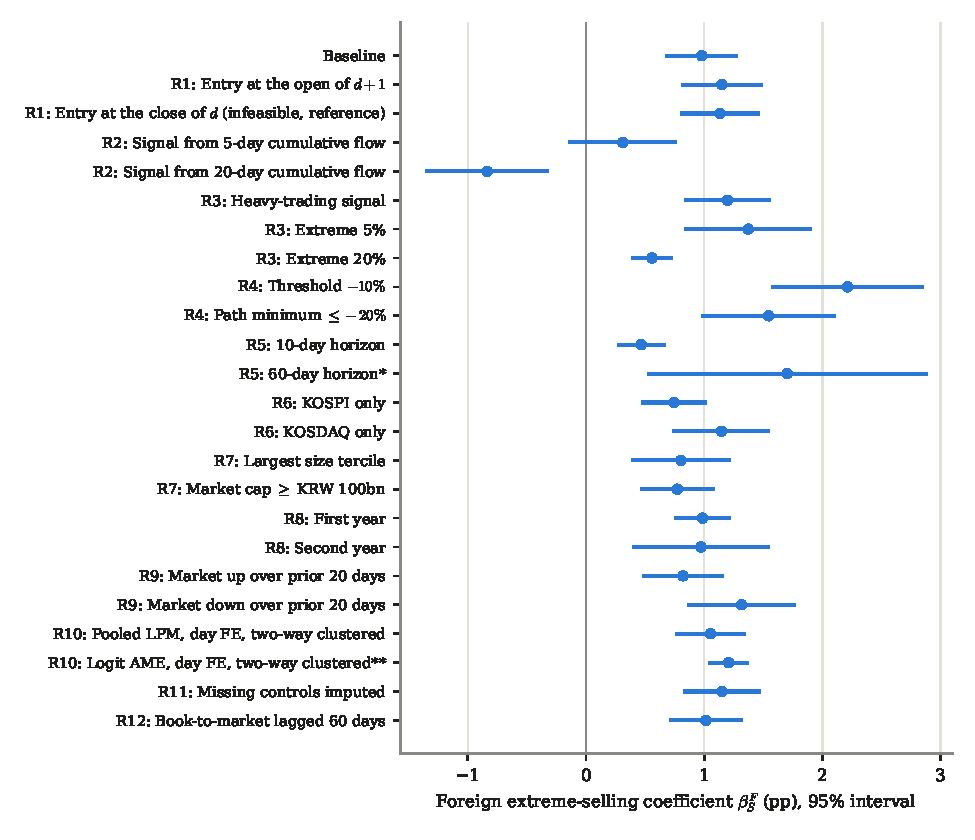
\includegraphics[width=0.95\textwidth]{figures/f2_forest.pdf}
\caption{Foreign extreme-selling coefficient across pre-specified specifications. Points are coefficients from
Table~\ref{tab:robust} (percentage points); bars are 95\% intervals based on the standard errors described there.
* underpowered; ** approximate standard errors.}\label{fig:forest}
\end{figure}

\subsection{Time and cross-sectional splits}
Panel A of Table~\ref{tab:split} splits the sample into its first and second years. The foreign-selling effect is
virtually identical in the two years (0.99 versus 0.97 points). The two asymmetries are not: the foreign
selling-minus-buying difference falls from 1.11 to 0.29 points and the individual buying-minus-selling difference from
1.54 to 0.36 points, and both declines are statistically significant ($p=0.007$ and $p=0.003$).
Figure~\ref{fig:rolling} shows the same pattern in 60-day rolling averages of the daily coefficients. Panel B splits the
cross-section into random halves 200 times. H1 is positive and significant in both halves in every split, H2 in
97.5\%, and H4 in 99.5\%, so no small group of stocks drives the results.

These splits use the data from which the hypotheses were derived and are not true out-of-sample tests. The analysis
plan therefore specifies a forward evaluation on signal days from 23 October 2026, with a first look after 60 and a
second after 120 signal days; the primary criterion is a one-sided $p<0.05$ for H2 at the second evaluation. If the
effect stays at its full-sample size the expected $t$-statistic after 120 days is about 2.4, but the second-year
decline in Panel A makes a failure of H2 a real possibility. H1 will be reported alongside it.

\begin{table}[htbp]\centering
\caption{Within-sample replication: time and cross-sectional splits}\label{tab:split}
\small
\textit{Panel A: First year versus second year}\\[3pt]
\begin{tabular}{lcccc}\toprule
 & First year & Second year & $z$ (difference) & $p$ (two-sided) \\\midrule
H1: Foreign $\beta_S$ & 0.99 (8.16) & 0.97 (3.27) & 0.04 & 0.964 \\
H2: Foreign $\beta_S-\beta_B$ & 1.11 (6.60) & 0.29 (1.16) & 2.69 & 0.007 \\
H4: Individual $\beta_B-\beta_S$ & 1.54 (5.81) & 0.36 (1.22) & 2.98 & 0.003 \\
H3: Institutional $\beta_S-\beta_B$ & 0.54 (2.40) & 0.28 (0.77) & 0.62 & 0.532 \\
\bottomrule\end{tabular}\\[8pt]
\textit{Panel B: Random halves of stocks, 200 splits}\\[3pt]
\begin{tabular}{lccccc}\toprule
 & Same sign in & Significant in & \multicolumn{3}{c}{$t$-statistics (400 halves)} \\
\cmidrule(lr){4-6}
 & both halves (\%) & both halves (\%) & Min & Median & Max \\\midrule
H1: Foreign $\beta_S$ & 100.0 & 100.0 & 3.03 & 5.07 & 9.07 \\
H2: Foreign $\beta_S-\beta_B$ & 100.0 & 97.5 & 1.20 & 3.20 & 5.28 \\
H4: Individual $\beta_B-\beta_S$ & 100.0 & 99.5 & 1.64 & 3.47 & 5.92 \\
\bottomrule\end{tabular}
\begin{minipage}{0.95\textwidth}\vspace{0.5em}\scriptsize
\textit{Notes:} Panel A re-estimates the baseline model separately for signal days 22 October 2024 to 22 October 2025 and 23 October 2025 to 17 September 2026 (coefficients in percentage points, signed so that positive values support the hypothesis; Newey--West $t$-statistics in parentheses). $z=(\bar\beta_1-\bar\beta_2)/\sqrt{se_1^2+se_2^2}$ treats the two halves as independent. Panel B splits the cross-section of stocks into two random halves (seeds 0--199) and re-estimates the baseline model in each half; ``significant'' means a one-sided $p<0.05$. Both panels use data from which the hypotheses were derived and are therefore not true out-of-sample tests.
\end{minipage}\end{table}

\begin{figure}[htbp]\centering
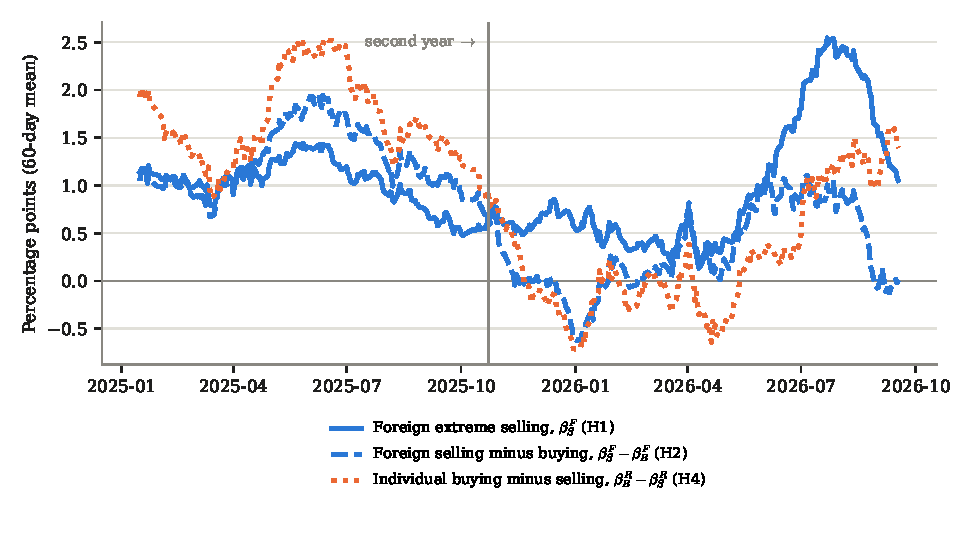
\includegraphics[width=0.95\textwidth]{figures/f1_rolling.pdf}
\caption{Rolling 60-signal-day averages of the daily cross-sectional coefficients from equation~\eqref{eq:lpm}, in
percentage points. The vertical line marks the start of the second year (23 October 2025).}\label{fig:rolling}
\end{figure}

\section{Discussion}\label{sec:discussion}

\subsection{Interpretation}
The evidence fits a simple account. On some days a group of investors with an informational or speed advantage---in this
sample, foreign investors---sells a stock aggressively relative to its size. The selling is absorbed largely by
individuals. The price does not fully adjust at once, and when the underlying news is bad the remaining adjustment
arrives as a large drop within weeks. Because such episodes are rare and mixed with many uninformative trades, the
average return of a portfolio sorted on flows barely moves, but the frequency of large losses does. This account is
consistent with theories in which bad news is accumulated and released abruptly \citep{jin2006}, and with evidence that
individual purchases are attention driven \citep{barber2008}. The finding that sustained, multi-week foreign selling is
not risky suggests that the informative component is the unusual one-day trade, not the trend.

The results do not establish causality. Foreign selling could cause subsequent declines through price pressure, or
foreign investors could simply anticipate declines; the regressions cannot separate the two. Nor is the signal a
precise forecasting tool: even among stocks with the strongest signals, more than 95\% do not experience a tail event
within 20 days.

\subsection{Implications for risk management}
For a long-only investor, the most direct use is in position sizing and monitoring. Heavy one-day foreign selling in a
held stock---especially when combined with heavy individual buying---raises the probability of a large relative loss
by roughly a third, after accounting for the stock's own volatility and recent price moves. That is relevant for
setting position limits, stop-loss levels, or review triggers. Institutional selling, often read as a negative signal,
is a much weaker marker. Conversely, nothing in the results supports using the same flows to forecast average returns
or market direction.

\subsection{Limitations}
The sample spans two years, a period in which the large-cap KOSPI rallied strongly and the KOSDAQ did not; the
asymmetry results weaken in the second year. The skewness-based outcomes are noisy over 20 days. Standard errors for
logit marginal effects are approximate. The investor-type data aggregate heterogeneous traders into three groups;
domestic institutions, in particular, combine pension funds, insurers, mutual funds, and proprietary desks with very
different motives. Finally, the hypotheses originated in exploratory work on the same data, so the in-sample tests are
confirmatory only in the limited sense that the specification was fixed in advance; the forward test is the real check.

\section{Analysis plan: deviations and disclosures}\label{sec:prereg}
The analysis plan was written on 27 October 2026 and stored with the code; it was not registered with an external
registry. The following deviations and disclosures apply.
\begin{enumerate}\itemsep2pt
\item During construction of the variables, and before the confirmatory regressions, a diagnostic printout displayed
the raw (uncontrolled) frequencies of the tail event by extreme-flow signal. The printout was removed and recorded in
the plan's change log; no hypothesis, variable, or test was changed.
\item An error in the first construction of beta (a missing value in the first index return propagated through rolling
sums) was found and fixed before any outcome-based analysis.
\item The wording of H8 did not anticipate significantly negative after-cost alphas; the formal outcome is reported as
planned (Section~\ref{sec:returns}).
\item The interpretations of the cumulative-flow, $-10\%$ threshold, and 60-day results (Section~\ref{sec:robust}) were
not anticipated in the plan and are labeled exploratory.
\end{enumerate}

\section{Conclusion}\label{sec:conclusion}
Korean investor-type flows, published daily for every stock, are a poor guide to average returns but a useful guide
to the left tail. Heavy one-day foreign selling raises the probability of a large one-month underperformance by about a
third, after controlling for the usual predictors of volatility and crashes, in both exchanges and in every random half
of the cross-section. Selling by foreign investors is riskier than their buying, and buying by individuals is riskier
than their selling, but these asymmetries weakened in the most recent year. A forward test on post-October 2026 data,
scheduled in the analysis plan, will show whether the results survive outside the sample in which they were found.

\begin{thebibliography}{99}\small
\bibitem[Amihud(2002)]{amihud2002} Amihud, Y. (2002). Illiquidity and stock returns: Cross-section and time-series effects. \textit{Journal of Financial Markets}, 5(1), 31--56.
\bibitem[Barber and Odean(2008)]{barber2008} Barber, B. M., and Odean, T. (2008). All that glitters: The effect of attention and news on the buying behavior of individual and institutional investors. \textit{Review of Financial Studies}, 21(2), 785--818.
\bibitem[Cameron et~al.(2011)]{cameron2011} Cameron, A. C., Gelbach, J. B., and Miller, D. L. (2011). Robust inference with multiway clustering. \textit{Journal of Business \& Economic Statistics}, 29(2), 238--249.
\bibitem[Carhart(1997)]{carhart1997} Carhart, M. M. (1997). On persistence in mutual fund performance. \textit{Journal of Finance}, 52(1), 57--82.
\bibitem[Chen et~al.(2001)]{chen2001} Chen, J., Hong, H., and Stein, J. C. (2001). Forecasting crashes: Trading volume, past returns, and conditional skewness in stock prices. \textit{Journal of Financial Economics}, 61(3), 345--381.
\bibitem[Choe et~al.(1999)]{choe1999} Choe, H., Kho, B.-C., and Stulz, R. M. (1999). Do foreign investors destabilize stock markets? The Korean experience in 1997. \textit{Journal of Financial Economics}, 54(2), 227--264.
\bibitem[Choe et~al.(2005)]{choe2005} Choe, H., Kho, B.-C., and Stulz, R. M. (2005). Do domestic investors have an edge? The trading experience of foreign investors in Korea. \textit{Review of Financial Studies}, 18(3), 795--829.
\bibitem[Fama and French(1993)]{fama1993} Fama, E. F., and French, K. R. (1993). Common risk factors in the returns on stocks and bonds. \textit{Journal of Financial Economics}, 33(1), 3--56.
\bibitem[Fama and MacBeth(1973)]{fama1973} Fama, E. F., and MacBeth, J. D. (1973). Risk, return, and equilibrium: Empirical tests. \textit{Journal of Political Economy}, 81(3), 607--636.
\bibitem[Griffin et~al.(2003)]{griffin2003} Griffin, J. M., Harris, J. H., and Topaloglu, S. (2003). The dynamics of institutional and individual trading. \textit{Journal of Finance}, 58(6), 2285--2320.
\bibitem[Grinblatt and Keloharju(2000)]{grinblatt2000} Grinblatt, M., and Keloharju, M. (2000). The investment behavior and performance of various investor types: A study of Finland's unique data set. \textit{Journal of Financial Economics}, 55(1), 43--67.
\bibitem[Harvey et~al.(2016)]{harvey2016} Harvey, C. R., Liu, Y., and Zhu, H. (2016). \ldots and the cross-section of expected returns. \textit{Review of Financial Studies}, 29(1), 5--68.
\bibitem[Holm(1979)]{holm1979} Holm, S. (1979). A simple sequentially rejective multiple test procedure. \textit{Scandinavian Journal of Statistics}, 6(2), 65--70.
\bibitem[Hutton et~al.(2009)]{hutton2009} Hutton, A. P., Marcus, A. J., and Tehranian, H. (2009). Opaque financial reports, $R^2$, and crash risk. \textit{Journal of Financial Economics}, 94(1), 67--86.
\bibitem[Jegadeesh(1990)]{jegadeesh1990} Jegadeesh, N. (1990). Evidence of predictable behavior of security returns. \textit{Journal of Finance}, 45(3), 881--898.
\bibitem[Jin and Myers(2006)]{jin2006} Jin, L., and Myers, S. C. (2006). $R^2$ around the world: New theory and new tests. \textit{Journal of Financial Economics}, 79(2), 257--292.
\bibitem[Kaniel et~al.(2008)]{kaniel2008} Kaniel, R., Saar, G., and Titman, S. (2008). Individual investor trading and stock returns. \textit{Journal of Finance}, 63(1), 273--310.
\bibitem[Kim and Wei(2002)]{kim2002} Kim, W., and Wei, S.-J. (2002). Foreign portfolio investors before and during a crisis. \textit{Journal of International Economics}, 56(1), 77--96.
\bibitem[Newey and West(1987)]{newey1987} Newey, W. K., and West, K. D. (1987). A simple, positive semi-definite, heteroskedasticity and autocorrelation consistent covariance matrix. \textit{Econometrica}, 55(3), 703--708.
\bibitem[Nosek et~al.(2018)]{nosek2018} Nosek, B. A., Ebersole, C. R., DeHaven, A. C., and Mellor, D. T. (2018). The preregistration revolution. \textit{Proceedings of the National Academy of Sciences}, 115(11), 2600--2606.
\bibitem[Petersen(2009)]{petersen2009} Petersen, M. A. (2009). Estimating standard errors in finance panel data sets: Comparing approaches. \textit{Review of Financial Studies}, 22(1), 435--480.
\bibitem[Richards(2005)]{richards2005} Richards, A. (2005). Big fish in small ponds: The trading behavior and price impact of foreign investors in Asian emerging equity markets. \textit{Journal of Financial and Quantitative Analysis}, 40(1), 1--27.
\bibitem[Schuirmann(1987)]{schuirmann1987} Schuirmann, D. J. (1987). A comparison of the two one-sided tests procedure and the power approach for assessing the equivalence of average bioavailability. \textit{Journal of Pharmacokinetics and Biopharmaceutics}, 15(6), 657--680.
\end{thebibliography}

\appendix
\section{Variable definitions}\label{app:vars}
\begin{small}
\begin{description}\itemsep1pt
\item[Net-buying intensity $x^j_{i,d}$.] Net purchase value of investor group $j$ (foreign; institutions; individuals)
in stock $i$ on day $d$, divided by the day-$d$ closing market capitalization. Zero if the group did not trade.
\item[Extreme signals $S^j$, $B^j$.] Bottom and top deciles of $x^j_{i,d}$ within the stock's exchange on day $d$.
Cumulative variants replace $N^j_{i,d}$ with the sum over the last $k=5$ or $20$ days. The heavy-trading variant sorts
stocks into size terciles, then into terciles of gross trading intensity (buy plus sell value over market cap) of group
$j$, and flags the bottom and top 30\% of $x^j$ within the highest-activity cell.
\item[Holding return $R^h_{i,d}$.] Compounded daily KRX return from the close of $d+1$ to the close of $d+1+h$.
Suspended days and days after delisting have zero return.
\item[Market-adjusted return $e^h_{i,d}$.] $R^h_{i,d}$ minus the equal-weighted mean of $R^h$ over all universe stocks on
the same exchange and signal day.
\item[Tail event $Y_{i,d}$.] One if $e^{20}_{i,d}\le-0.20$. Path-minimum variant: one if the lowest cumulative raw return
over the 20 days after entry is $-20\%$ or worse.
\item[NCSKEW, DUVOL.] Computed from $w_{i,t}=\ln(1+r_{i,t}-\hat\beta_{i,d}r_{m,t})$ over the holding window
(minimum 15 of 20 or 45 of 60 observations): $\mathrm{NCSKEW}=-n(n-1)^{3/2}\sum w^3/[(n-1)(n-2)(\sum w^2)^{3/2}]$;
$\mathrm{DUVOL}=\ln[(n_u-1)\sum_{\text{down}}w^2/((n_d-1)\sum_{\text{up}}w^2)]$, where down (up) days have $w$ below
(above) the window mean.
\item[Controls.] Size: log market capitalization. Value: log of book value per share over price (missing if book value
is non-positive). Momentum: cumulative return over trading days $d-251$ to $d-21$. Reversal: cumulative return over
$d-20$ to $d-1$. Signal-day and entry-day returns: $r_{i,d}$, $r_{i,d+1}$. Volatility: standard deviation of daily
returns over $d-19$ to $d$. Beta: slope of daily returns on the exchange index over 250 days (minimum 120). Amihud:
mean of $|r|$ divided by trading value (KRW 100 million) over 20 days. Turnover: mean trading value over market cap over
20 days. Past NCSKEW: as above over $d-59$ to $d$.
\end{description}
\end{small}

\section{Additional tables}\label{app:tables}
\begin{table}[htbp]\centering
\caption{Investor flows and conditional skewness}\label{tab:crash}
\scriptsize\setlength{\tabcolsep}{3pt}
\begin{tabular}{lccccccccc}\toprule
 & \multicolumn{3}{c}{Foreign} & \multicolumn{3}{c}{Institutional} & \multicolumn{3}{c}{Individual} \\
\cmidrule(lr){2-4}\cmidrule(lr){5-7}\cmidrule(lr){8-10}
Dependent variable & $\beta_S$ & $\beta_B$ & $\beta_S-\beta_B$ & $\beta_S$ & $\beta_B$ & $\beta_S-\beta_B$ & $\beta_S$ & $\beta_B$ & $\beta_S-\beta_B$ \\\midrule
NCSKEW, 20 days & 0.005 & 0.002 & 0.003 & -0.006 & -0.018 & 0.012 & 0.012 & 0.010 & 0.001 \\
 & (0.42) & (0.15) & (0.37) & (-0.39) & (-1.61) & (1.07) & (0.91) & (0.83) & (0.12) \\[2pt]
DUVOL, 20 days & -0.000 & -0.005 & 0.004 & -0.033 & -0.038 & 0.005 & 0.008 & 0.003 & 0.005 \\
 & (-0.03) & (-0.33) & (0.44) & (-2.04) & (-3.07) & (0.47) & (0.57) & (0.24) & (0.41) \\[2pt]
NCSKEW, 60 days$^\dagger$ & 0.029 & 0.012 & 0.017 & 0.051 & 0.027 & 0.024 & 0.006 & 0.032 & -0.026 \\
 & (1.56) & (0.78) & (2.16) & (4.17) & (1.65) & (1.88) & (0.40) & (1.69) & (-2.63) \\[2pt]
DUVOL, 60 days$^\dagger$ & 0.008 & -0.003 & 0.010 & -0.011 & -0.016 & 0.006 & -0.003 & 0.007 & -0.010 \\
 & (0.48) & (-0.19) & (2.25) & (-0.97) & (-1.19) & (0.77) & (-0.23) & (0.48) & (-1.92) \\[2pt]
\bottomrule\end{tabular}
\begin{minipage}{0.95\textwidth}\vspace{0.5em}\scriptsize
\textit{Notes:} Same daily cross-sectional regressions as Table~\ref{tab:tail} with the dependent variable replaced by the negative coefficient of skewness (NCSKEW) or the down-to-up volatility ratio (DUVOL) of firm-specific log returns over the holding window. Firm-specific returns are $\ln(1+r_{i,t}-\hat\beta_{i,d}r_{m,t})$ with $\hat\beta$ estimated before the signal day. Newey--West $t$-statistics in parentheses. $^\dagger$426 signal days; seven non-overlapping windows.
\end{minipage}\end{table}
\begin{table}[htbp]\centering
\caption{Constructed Korean factors}\label{tab:factors}
\small
\begin{tabular}{lccc}\toprule
Factor & Days & Mean daily return (\%) & Annualized volatility (\%) \\\midrule
MKT & 485 & 0.161 & 41.1 \\
SMB & 485 & -0.151 & 18.8 \\
HML & 485 & -0.026 & 26.5 \\
MOM & 485 & 0.071 & 25.8 \\
STR & 485 & -0.003 & 27.3 \\
\bottomrule\end{tabular}
\begin{minipage}{0.85\textwidth}\vspace{0.5em}\scriptsize
\textit{Notes:} Factors are built from the study universe (both markets pooled). MKT is the value-weighted universe return minus the daily CD (91-day) rate; SMB and HML use a $2\times3$ sort on size (median) and book-to-market (30/70), MOM a $2\times3$ sort on 12--1 month returns, both reformed at month-ends; STR is a daily-reformed $2\times3$ sort on the prior 20-day return (losers minus winners). Correlations of daily returns with KRX indices: our KOSPI index 1.0000, our KOSDAQ index 0.9996; SMB with the average of (KOSPI small $-$ large) and (KOSDAQ small $-$ large) size indices 0.66. The lower SMB correlation reflects pooled-median versus within-market rank breakpoints.
\end{minipage}\end{table}

\end{document}
